\documentclass{article}

\usepackage{PRIMEarxiv}

\usepackage[utf8]{inputenc} % allow utf-8 input
\usepackage[T1]{fontenc}    % use 8-bit T1 fonts
\usepackage{hyperref}       % hyperlinks
\usepackage{url}            % simple URL typesetting
\usepackage{booktabs}       % professional-quality tables
\usepackage{amsmath}        % equations
\usepackage{amsfonts}       % blackboard math symbols
\usepackage{amssymb}        % extra math symbols
\usepackage{bm}             % bold math
\usepackage{nicefrac}       % compact symbols for 1/2, etc.
\usepackage{microtype}      % microtypography
\usepackage{fancyhdr}       % header
\usepackage{graphicx}       % graphics
\usepackage{xcolor}         % placeholders in red
\usepackage{algorithm}      % Algorithm 1
\usepackage{algpseudocode}
\graphicspath{{figures/}}   % figures live in figures/

% Placeholders: [TBD: ...] marks a result or text that does not exist yet, [CITE? ...] a reference not yet saved.
\newcommand{\tbd}[1]{\textcolor{red}{[TBD: #1]}}
\newcommand{\citeq}[1]{\textcolor{red}{[CITE? #1]}}

% Header
\pagestyle{fancy}
\thispagestyle{empty}
\rhead{ \textit{ }}
\fancyhead[LO]{Protective-Field Barrier Filtering of Field-Blind Local Planners (draft)}

%% Title
\title{Protective-Field Barrier Filtering of Field-Blind Local Planners under a Certified Safety Layer
\thanks{\textit{\underline{Status}}: draft, not submitted. Placeholders in red mark results and references that do not exist yet.}
}

\author{
  Author One, Author Two \\
  Affiliation \\
  City, Country \\
  \texttt{\{author1, author2\}@example.org} \\
}

\begin{document}
\maketitle

\begin{abstract}
Autonomous mobile robots in warehouses share aisles with people, and an independent certified laser scanner protects them with a speed-banded field whose breach latches a stop. Navigation software that does not account for this field triggers such stops repeatedly, and each one costs a restart delay or a deadlock. This paper proposes the Protective-Field Barrier, a discrete-time barrier filter on the sectors of the laser scan, whose field mirrors the certified layer and which returns the command closest to the controller's request that keeps every valid return outside the field. The filter sits between a local controller and an emulated certified layer, which stays active, and is the identity when switched off. It is evaluated beneath three field-blind classical planners, pure pursuit, regulated pure pursuit and a holonomic dynamic window planner, on warehouse routes with and without an unmapped obstacle. In exploratory validation runs the filter removes nearly all protective stops and every unrecoverable stop. For the dynamic window planner, the strongest of the three, stops per 100 m of planned route fall from 8.35 to 0.0 on routes without an unmapped obstacle and from 45.7 to 0.0 on routes with one. With an unmapped obstacle on every route, however, most routes end in timeouts, because the stack does not replan. These results indicate that the filter removes the avoidable stops of controllers that ignore the protective field, while stop removal alone does not complete such routes. A sealed test set confirms the stop reduction for regulated pure pursuit.
\end{abstract}

\keywords{Protective field \and Control barrier function \and Certified safety layer \and Mobile robot \and LiDAR}

\section{Introduction}

Autonomous mobile robots (AMRs) in warehouses move through aisles they share with people. Their safety does not rest on the navigation software. An independent certified safety function monitors a protective field around the vehicle with a safety laser scanner and commands a stop when an object enters it \cite{iso3691-4,iec61496-3}. The field depends on the speed and direction of travel, and the stop latches until the field is clear and a restart condition holds. Production robots keep such certified scanners because software safety is hard to demonstrate to a safety body, and conservative fields can cause frequent stopping~\cite{liu2017}. Industrial studies of these fields measure their efficiency by fewer slowdowns and stops~\cite{muhammad2021}.

The navigation software above this layer is not certified, and it typically optimises navigation objectives without explicitly accounting for the geometry and the speed-dependent switching of the certified fields. Classical local planners represent obstacles by an inflation radius or a clearance cost \cite{coulter1992purepursuit,macenski2023rpp,fox1997dwa}. Such a planner treats the certified field as an unknown region of the world, so nothing in its design keeps the robot out of it. A planner can therefore be collision-free in its own terms and still trigger a stop at shelf corners, in narrow aisles and next to obstacles that are missing from its map. Protective stops are essential safety responses to detected intrusions. Some of them, however, arise from a mismatch between the nominal commands and the modeled field geometry, and not from an unavoidable collision situation: an oracle tracker with privileged knowledge can traverse every route of our scenario sets without breaching the lowest band's field (Section 5.2). Such stops are avoidable operational interruptions, and reducing them while the certified layer stays independent and active is the aim of this paper. Figure~\ref{fig:motivation} shows one such stop and the filtered alternative on a tuning scenario. Each trigger costs a restart delay and, in the worst case, a deadlock in which the restart condition never clears. On a certified vehicle the layer itself largely bounds collisions, so the operational cost that remains is the protective stop. We therefore take protective stops per 100 m of planned route as the primary metric, and report success, timeouts and mission time beside it, because a controller can lower its stop count by moving little.

\begin{figure}[t]
\centering
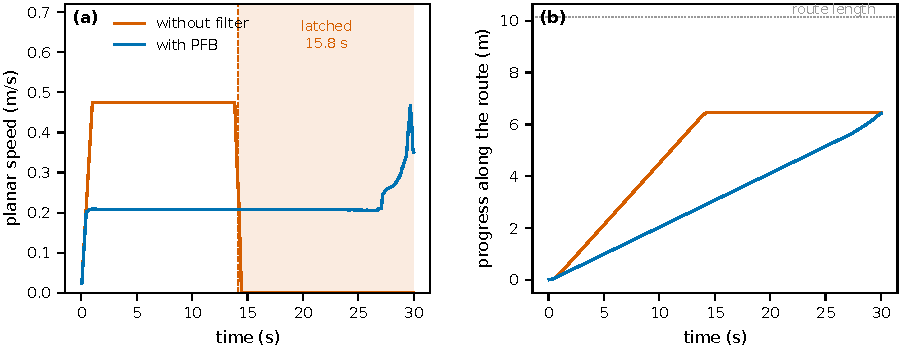
\includegraphics[width=\linewidth]{fig_motivation.pdf}
\caption{The operational cost of one protective stop, in an emulated run on the first narrow-aisle tuning scenario (planned route 10.1~m). A scan-blind route tracker, used only as an illustrative requested-command generator, drives the route twice with the certified layer beneath it. Without the filter it triggers one protective stop at 14~s (dashed line), and the latch (shaded) does not release within the 30~s window, because the declared recovery is not part of this emulation. With the PFB it triggers no stop but moves at a lower speed, and neither run reaches the goal within the window. (a) Planar speed. (b) Progress along the planned route.}
\label{fig:motivation}
\end{figure}

Control barrier functions (CBFs) constrain a command so that a safe set stays forward invariant \cite{ames2017cbfqp}. Used as a safety filter, a small quadratic program (QP) returns the admissible command closest to the one a controller requested. Filters of this kind are well established. Beam-wise discrete-time barrier constraints on LiDAR returns have been used with a constant safety margin~\cite{olayemi2026}. Filters of this kind can also stall a robot at undesired equilibria~\cite{mestres2026}. In the filters we reviewed, the safe set is a clearance chosen by the designer~\cite{olayemi2026}, and not the geometry and speed-regime switching of an external protective-field system. We do not claim a new barrier function, and the filter we use belongs to this family.

Among the works we reviewed, none protects a latching, speed-banded certified layer with a restart condition, and none evaluates a filter in that layer's own cost, protective stops, across controllers. This paper studies that case for classical local planners that do not account for the certified field, which we call field-blind. We evaluate three of them, pure pursuit, regulated pure pursuit and a holonomic dynamic window planner, and treat the dynamic window planner as the lead case, since it is the strongest of the three. We use the Protective-Field Barrier (PFB), a discrete-time barrier filter defined on the sectors of the laser scan, whose field mirrors the speed-banded protective field of the certified layer. The PFB sits between any controller and the layer. The filter modifies the nominal command to satisfy a one-step protective-field exclusion constraint under the assumed robot and sensing models: over one prediction horizon, no valid scan return may lie inside the modeled protective field of the speed regime the robot will be in. The filter solves one QP per speed regime for a holonomic base, brakes at the maximum rate when no regime is feasible, and is the identity when switched off. It is a candidate barrier: we do not show that it is a valid CBF, and we claim no safety guarantee beyond the emulated layer. The filter does not replace the certified layer, which remains independent and active.

The contributions are as follows.

\begin{itemize}
\item \emph{Methodological.} A protective-field-aware filtering formulation. The PFB places a barrier field that mirrors the speed-banded field of the certified layer between a controller and that layer, for a holonomic base with wheel-speed and acceleration limits, as an application of beam-wise discrete-time LiDAR barrier filters (Section 4).
\item \emph{Integration.} A controller-independent placement of the filter beneath three field-blind classical local planners, with the filter as the identity when switched off, so that a controller with and without it differs in one respect (Section 4).
\item \emph{Experimental.} A paired evaluation of protective stops, an explicit operational metric, beside success, timeouts and mission time, with an emulated certified layer beneath every controller. It establishes where the filter removes avoidable stops of field-blind planners and where it leaves routes incomplete when an obstacle is missing from the map, and it adds the sensitivity of the stops to the barrier gain (Sections 5 and 6). The results on the validation sets are exploratory, and the confirmatory comparison HF-c on the sealed test set covers regulated pure pursuit (Sections 5.6 and 6.2) \tbd{Section 6.4}
\end{itemize}

Section 2 reviews related work. Section 3 gives the preliminaries and the problem statement, Section 4 the filter and the controllers it sits beneath, Section 5 the experimental design, Section 6 the results, Section 7 the discussion, Section 8 the future work, and Section 9 concludes.


\section{Related Work}

This section reviews work on the safety fields of industrial robots (2.1), classical local planners (2.2), barrier filters for LiDAR navigation (2.3), and the stalls that barrier filters can cause (2.4). Subsection 2.5 states how this paper relates to that work.

\subsection{Industrial safety fields}

Driverless industrial vehicles are governed by safety standards, and their personnel and obstacle detection is provided by certified safety laser scanners \cite{iso3691-4,iec61496-3} \cite{tiusanen2020}. At the lowest performance level, a vehicle has a static protection field with a discretised warning field, and the efficiency of the arrangement is read as fewer slowdowns and stops. Muhammad et al.~\cite{muhammad2021} adapt the warning field itself and evaluate it on one 510 m trajectory. Liu et al.~\cite{liu2017} observe that production robots still rely on certified laser scanners because software safety is hard to demonstrate to a safety body, and that conservative circular fields cause frequent stopping. They propose reachability-based safe motion among pedestrians and read efficiency as average speed. In both works the protective field is given or reshaped, and neither couples it to a barrier filter on the navigation command. Neither counts protective stops with numbers.

\subsection{Classical local planners}

Local planners that track a global route include pure pursuit, regulated pure pursuit and the dynamic window approach \cite{coulter1992purepursuit,macenski2023rpp,fox1997dwa}. They represent obstacles by an inflation radius, a clearance term or a cost, chosen by the designer. Barrier constraints have also been built into planners themselves, in which a barrier filter acts on each sampled rollout and on the executed command~\cite{coker2026}. Our approach keeps the planner unchanged and wraps it, so that the same filter applies to any planner.

\subsection{Barrier filters on LiDAR returns}

Control barrier functions (CBFs) constrain a command so that a safe set stays forward invariant, and a quadratic program (QP) selects the admissible command closest to the requested one \cite{ames2017cbfqp}. For discrete-time systems the condition is imposed on one step, $h_{k+1} \ge (1 - \gamma \Delta t)\,h_k$~\cite{yang2026cbfrl}.

The closest prior art to our filter applies this condition beam by beam to LiDAR returns. Olayemi et al.~\cite{olayemi2026} define a perception-aware CBF with a constant safety margin of 0.3 m, a QP with slack, a unicycle model, 32 forward beams, a range-rate estimate and a constant-input predictive extension. They report collisions over 100 episodes in one table, for no filter, the CBF, an instantaneous version and a predictive version. Their margin does not depend on speed or direction, and they have no certified layer, no stop metric, and no seeds or intervals. The Protective-Field Barrier (PFB) uses a row of the same discrete-time form as this filter. It differs in the field: it is continuous in direction and yaw rate and piecewise in speed, it is built from the certified layer's own configuration, and it acts on a holonomic base with wheel-speed and acceleration limits. Its field mirrors the layer, and the evaluation counts the layer's stops.

\subsection{Stalls caused by barrier filters}

Mestres et al.~\cite{mestres2026} show that continuous-time CBF filters can have undesired equilibria, locally stable even for convex safe sets, and limit cycles in dimension above two that tuning the parameters cannot always remove. Our filter is discrete and sits above a latch, so their analysis explains stalls only by analogy. We report timeouts beside stops for this reason.

\subsection{Position}

Filters on LiDAR returns are published. We do not claim them. Among the works we reviewed, none protects a latching, speed-banded certified layer with a restart condition, none uses that layer's protective stops as its metric, and none evaluates one filter beneath several classical planners. This paper contributes that application and its evaluation for classical planners, together with a sensitivity analysis of the barrier gain and a report of the stalls that the filter can cause. Learned planners are left to future work.

\section{Preliminaries and Problem Statement}

We first fix the interface of a controller, then describe the certified safety layer that runs beneath every controller, then state the discrete-time barrier condition that a safety filter enforces. The last subsection states the problem.

\subsection{Controllers}

The robot is commanded by a planar body-frame velocity $u = (v_x, v_y, \omega)$ of a holonomic base, with forward speed $v_x$ and lateral speed $v_y$ in m/s and yaw rate $\omega$ in rad/s. The control period is $\Delta t = 0.05$ s. A \emph{controller} maps its inputs, the scan, a lookahead point on the route and the goal, to a nominal command $u_{\mathrm{nom}}$. The controllers in this paper are classical: each computes $u_{\mathrm{nom}}$ from the route and the scan by a fixed rule (Section 4.3). An episode ends when the robot reaches the goal within 0.25 m, when the simulator reports a contact, or when 4,000 steps (200 s) have elapsed. Collisions are defined only by the simulator's contact check and never by a LiDAR threshold. The method does not depend on the form of the controller, because the filter acts on the command alone.

\subsection{The certified safety layer}

Industrial mobile robots are protected by a safety function that is certified independently of navigation \cite{iso3691-4,iec61496-3}. We emulate such a layer in simulation. It has three properties. First, it is independent: it uses its own sensing channel, a safety laser scanner, and shares no logic or tuning with the controller it supervises. Second, its protective fields are fixed and declared in advance. The trigger set is a finite family of regions, selected by a discrete speed band and by the direction of travel, and it is not computed from the controller's intent. Third, its only action is to stop. The emulation does not claim functional-safety compliance. In this paper a protective stop is an event of this emulated layer, a modeled protective stop, and not a measurement of a physical certified device.

Let $P_k$ denote the valid scan points in the body frame, $\hat v_k$ the velocity estimate, $b_k$ the speed band selected by the speed the robot can reach within one response time, and $\mathcal{F}(b, \vartheta)$ the closed region protected in band $b$ for travel direction $\vartheta$: the footprint swept along the braking segment, plus margins. The layer is a latched state machine,

\begin{equation*}
\begin{aligned}
\mathrm{trig}_k &= \mathbf{1}\big[\exists\, p \in P_k:\ p \in \mathcal{F}(b_k, \vartheta_k)\ \text{or an invalid scan bin exists}\big],\\
\mathrm{lat}_k &= \mathrm{trig}_k \ \vee\ \big(\mathrm{lat}_{k-1} \wedge \neg\,\mathrm{rst}_k\big),
\end{aligned}
\tag{1}
\end{equation*}

whose output is a braking command (limited by the deceleration $a_{\mathrm{brake}}$) while $\mathrm{lat}_k$ holds and the commanded velocity otherwise. The restart condition $\mathrm{rst}_k$ holds when the field has been clear for the restart delay and no breaching point approaches the robot, that is $\hat v \cdot p \le 0$ for every breaching point $p$. An invalid scan bin is treated as an obstacle at the footprint boundary on its bearing, so unobserved space is never read as free. A \emph{protective stop} is one entry into the latched state of the emulated layer: a step at which the field in force is breached while no stop is triggered or latched. A breach that persists, and the latch that follows it, count as one stop. A breach after a restart counts as a new stop. Stops decided on a corrupted scan packet that was replaced by the fail-safe are excluded from the count and reported separately.

In our configuration the response time is 0.10 s, $a_{\mathrm{brake}} = 1.0$ m/s$^2$, the restart delay is 2.0 s, and the three bands have top speeds of 0.10, 0.30 and 0.51 m/s. The ahead margin is 0.10 m and the lateral margin 0.05 m. These values are configured, and the band speeds are not measured quantities. The layer runs beneath every controller. Because its fields are discrete and sized for the worst case of each band, it can stop a robot whose command a continuous analysis would show to be safe. Each such stop costs at least the restart delay.

\subsection{Barrier functions and the discrete-time condition}

Let $h$ be a continuously differentiable function of a reduced state $q$, and let $\mathcal{S} = \{q : h(q) \ge 0\}$ be the safe set. For a control-affine system $\dot q = f(q) + g(q)u$, the function $h$ is a control barrier function (CBF) on $\mathcal{S}$ if there is an extended class-$\mathcal{K}$ function $\alpha$ with $\sup_u [L_f h(q) + L_g h(q)\,u] > -\alpha(h(q))$ on $\mathcal{S}$. A controller that keeps the input in the set $\{u : L_f h + L_g h\, u \ge -\alpha(h)\}$ renders $\mathcal{S}$ forward invariant \cite{ames2017cbfqp}.

A controller acts at a fixed period, so we use the discrete-time condition. For $q_{k+1} = F(q_k) + G(q_k)u_k$, the function $h$ is a discrete-time CBF on $\mathcal{S}$ if for every $q \in \mathcal{S}$ some admissible $u$ satisfies

\begin{equation*}
h\big(F(q) + G(q)\,u\big) \ \ge\ \rho\, h(q), \qquad \rho \in [0, 1].
\tag{2}
\end{equation*}

Repeated use of (2) keeps $h$ above the geometrically decaying curve $\rho^{k} h(q_0)$~\cite{yang2026cbfrl}, following the discrete-time CBF literature. We write $\rho = 1 - \alpha \Delta t$ with $0 < \alpha \Delta t \le 1$. With $\alpha = 1.0$ s$^{-1}$ and $\Delta t = 0.05$ s, as in our experiments, $\rho = 0.95$.

A safety filter turns (2) into a quadratic program (QP) that changes the controller's nominal command as little as possible:

\begin{equation*}
u^{\ast} = \arg\min_{u \in \mathcal{U}_{\mathrm{adm}}}\ (u - u_{\mathrm{nom}})^{\top} W\,(u - u_{\mathrm{nom}})
\quad \text{s.t.}\quad h\big(q_{k+1}(u)\big) \ \ge\ (1 - \alpha \Delta t)\, h(q_k).
\tag{3}
\end{equation*}

When the constraint is inactive, $u^{\ast} = u_{\mathrm{nom}}$. CBF-RL~\cite{yang2026cbfrl} shows that for a single-integrator model the nonlinear discrete condition can be replaced by the continuous-time first-order condition, up to a bound that vanishes with the step, which yields a closed-form filter. We do not use that result. In our setting the predicted state depends on $u$ through a reach horizon, and the filter solves one QP per speed regime (Section 4).

Two limits apply. First, satisfying the constraint establishes compatibility with the modeled field at the predicted state. It does not establish continuous-time exclusion from the field over the whole subsequent trajectory, and it holds relative to the model: a kinematic prediction, a bounded estimation lag and the declared actuation limits. How well the approximation works depends on the accuracy of the motion model and of the sensing, on the control interval and on the representation of the speed-band switching, and it says nothing about the real world. For the candidate barrier studied here we do not show that it is a valid CBF, and we claim no safety guarantee. The independent certified layer therefore remains necessary and active. Second, when the QP is infeasible, no invariance claim holds for that step. The filter then brakes at the maximum rate, and the event is counted and reported (Section 4.2).

\subsection{Problem statement}

The robot receives a global route from an A$^{*}$ planner on a map that may omit obstacles. A controller receives the LiDAR scan with validity flags, a lookahead point on the route and the goal, and outputs $u_{\mathrm{nom}}$. The command that reaches the actuators is

\begin{equation*}
u = \mathcal{C}\big(\mathcal{P}(u_{\mathrm{nom}})\big),
\tag{4}
\end{equation*}

where $\mathcal{P}$ is the protective-field filter, the identity when it is disabled, and $\mathcal{C}$ is the certified layer (1). Let $N_{\mathrm{stop}}$ be the number of protective stops in an episode and $L_{\mathrm{plan}}$ the length of its planned route. The primary quantity is the rate

\begin{equation*}
\sigma = 100\, \frac{N_{\mathrm{stop}}}{L_{\mathrm{plan}}} \quad \text{(stops per 100 m of planned route)},
\tag{5}
\end{equation*}

computed over a set of scenarios. It normalises the number of modeled protective stops by the spatial extent of the task and gives an operational measure of how often the field intervenes. We divide by the planned length rather than the distance driven so that a controller cannot lower its rate by wandering, and the planned length is the same for every controller. A controller can also lower $\sigma$ by not moving, and a filter can stall a robot (Section 2.4). Success, timeouts and mission time are therefore reported beside $\sigma$.

The aim is not to eliminate protective stops, which are essential safety responses, but to reduce avoidable interruptions while the certified layer stays independent and active. The problem is to determine, for each controller, how much the filter $\mathcal{P}$ reduces $\sigma$ without reducing success. The next section describes the filter and the controllers it sits beneath.

\section{Method}

This section describes the Protective-Field Barrier (PFB) filter (4.2), the classical controllers beneath which it is placed (4.3) and a planned comparator filter (4.4).

\subsection{Overview}

Figure~\ref{fig:chain} shows the control chain of Eq. (4). The A$^{*}$ planner supplies a route on the map, which may omit obstacles. A classical controller proposes a nominal command $u_{\mathrm{nom}}$. The PFB filter replaces it by the closest command that keeps every valid scan return outside the protective field of the regime the robot will be in. The certified layer then passes this command or stops the robot, and the actuation limits (axis box, wheel-speed budget, acceleration limiter) apply last. With the filter disabled, $\mathcal{P}$ is the identity, so a controller without it is exactly the unfiltered controller. Every comparison in this paper differs in one respect: whether the filter sits between the controller and the certified layer.

\begin{figure}[t]
\centering
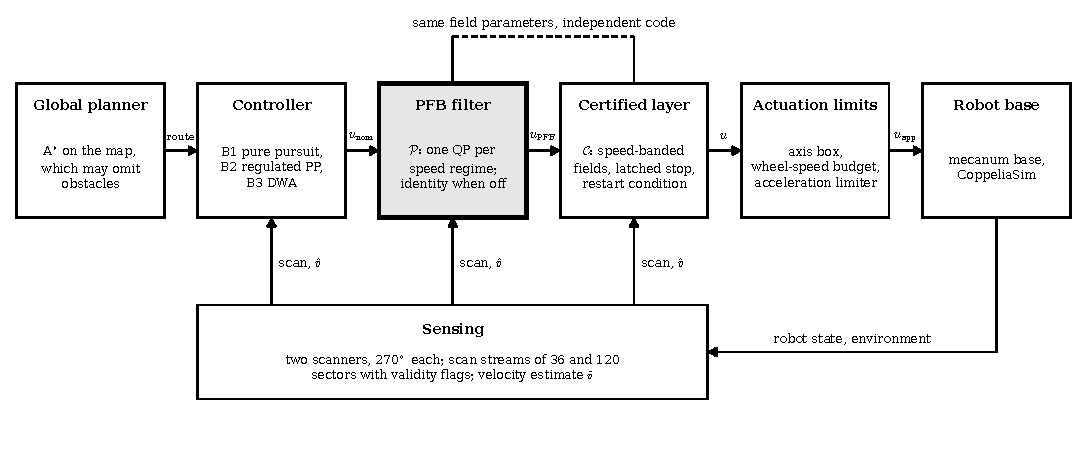
\includegraphics[width=\linewidth]{fig1_architecture.pdf}
\caption{Control chain of the proposed system. A global A$^*$ planner supplies a route on a map that omits some obstacles. A classical controller (B1, B2 or B3) maps the scan, the route lookahead and the goal to a nominal velocity command $u_{\mathrm{nom}}$. The Protective-Field Barrier (PFB) replaces $u_{\mathrm{nom}}$ by the closest command that keeps every valid scan return outside the protective field it will be in, and the certified layer then passes this command or applies a latched stop. The command $u$ drives the robot base in the simulator, whose state is read by the sensing block. The PFB and the certified layer use the same field parameters but independent code. With the filter switched off, the PFB is the identity. The shaded block is the proposed filter, $\mathcal{P}$ and $\mathcal{C}$ are the maps of Eq.~(4), and $u_{\mathrm{app}}$ is the command after the actuation limits.}
\label{fig:chain}
\end{figure}

\subsection{The Protective-Field Barrier filter}

\emph{Safe set.} The certified layer triggers when a valid scan point lies inside its field for the current band (1). The PFB takes the complement of that trigger region, with the discrete band fields replaced by a continuous protective field $\rho$ that depends on the command. Let $u = (v_x, v_y, \omega)$ be a candidate command and $\tau = \Delta t + \ell$ the prediction horizon, where $\ell = 0.05$ s is a lag allowance for the estimation delay. For the $i$-th valid scan return, let $r_i(u)$ and $\psi_i(u)$ be its range and bearing in the body frame after the robot has travelled at $u$ for $\tau$. The barrier row of return $i$ is

\begin{equation*}
g_i(u) = r_i(u) - \rho\big(\psi_i(u);\, \theta(u),\, W(u)\big) - \delta,
\tag{6}
\end{equation*}

and the candidate discrete-time condition (cf. (2) and (3)) is

\begin{equation*}
g_i(u) \ \ge\ (1 - \alpha \Delta t)\,\max\big(h_i^{\mathrm{now}},\, 0\big) \quad \text{for every valid return } i,
\tag{7}
\end{equation*}

where $h_i^{\mathrm{now}}$ is the same quantity at the current state. The function $\rho(\psi; \theta, W)$ is the distance from the robot to the boundary of the protective field along bearing $\psi$. The field is the footprint swept over the heading change reachable in $\tau$, extended along the heading $\theta(u)$ of the command by the distance travelled over the reach time plus the braking distance, $D(V) = V T + V^2 / (2 a_{\mathrm{brake}})$, and by margins. The heading $\theta(u)$ follows the command where it dominates the velocity estimate, and $W(u) = \max(|\hat\omega|, |\omega|)$ is the yaw rate for which the field is swept. The offset $\delta$ is the measured binning penalty of the scan at its upper bound (0.5 mm). Because the field is built from the same configuration as the certified layer but by independent code, the two cannot drift apart silently. The row has the discrete-time, beam-wise form of earlier LiDAR barrier filters~\cite{olayemi2026}. It differs from a constant-margin row in that the field depends on the speed and direction of the command and on the yaw rate. Figures~\ref{fig:fields} and~\ref{fig:step} show the fields and one filter step.

Taking the maximum with zero in (7) fixes the behaviour at a breached regime. If a return is already inside the field of the regime the robot would be in, the filter requires it to be clear after one step, and it never lets the robot enter a breached regime from outside. As stated in Section 3.3, $h_i$ is a candidate barrier whose validity is not established.

\emph{Assumptions and limits.} The condition (7) is evaluated over one prediction horizon $\tau = 0.10$ s, on a grid of five motion fractions of the predicted motion, with each row tightened by a margin so that the minimum over the grid bounds the minimum over the whole horizon. Satisfying it establishes compatibility with the modeled field over this horizon. It does not establish continuous-time exclusion from the field over the rest of the trajectory. Its effectiveness depends on the accuracy of the kinematic model, the validity of the range measurements, the control interval and the representation of the speed-band switching. Table~\ref{tab:field} lists the field model and the filter parameters, and Figure~\ref{fig:flowchart} summarises one decision of the filter. The emulated field reproduces the structure of a speed-banded, latching protective-field system, with the footprint swept along the braking segment plus margins. It is not the configuration of a specific commercial device. The independent certified layer therefore remains necessary and active.

\emph{Quadratic program.} For each speed regime of the certified layer (the at-rest field, or the band selected by the reachable speed), the filter solves

\begin{equation*}
\min_{u}\ (u - u_{\mathrm{nom}})^{\top}\, \mathrm{diag}(1, 1, \rho_{\mathrm{out}}^{2})\,(u - u_{\mathrm{nom}})
\quad \text{s.t. (7) for all } i,\ \ u \in \mathcal{U}_{\mathrm{adm}},\ \ \text{speed within the regime}.
\tag{8}
\end{equation*}

The weight $\rho_{\mathrm{out}} = 0.3374$ m, the outer radius of the footprint, converts a yaw rate into the speed of the footprint's outermost point, so that translation and rotation are penalised in the same units. The admissible set contains the mecanum wheel-speed polytope, the axis box, and the one-step envelope of the acceleration limiter. The rows (7) are nonlinear in $u$. They are linearised, with tangent planes in the translation and chords in the yaw rate, and each row more than 0.5 m from binding is left out of the QP. The true rows are checked at the solution with no tolerance, and one re-linearisation is allowed. The best feasible regime wins. A regime is infeasible when its QP has no solution, or when the true rows, checked at the solution with no tolerance, are violated after the allowed re-linearisation. If no regime is feasible, the filter issues the maximum-braking command, within the acceleration limiter, and labels the step infeasible; these steps are counted and reported. Braking is a fallback and not a regular control response. It does not guarantee that the predicted field constraint holds or that the certified layer will not trigger: the layer stays active and can still latch a stop on that step or the next.

\emph{Under the latch.} While the certified layer is latched, only a command that its restart condition could release passes: a creep that recedes from every point inside the at-rest field, or a twist whose own band field is clear. Otherwise the output is zero. The filter never removes or weakens the certified layer, which remains the backstop.

\emph{Gain.} The gain $\alpha$ is frozen at 1.0 s$^{-1}$ for every filtered controller. This is the lowest value of the grid searched on the tuning scenarios, and we do not claim it is optimal. The effect of $\alpha$ on the stops is reported as a sensitivity result (Section 6.3).

\emph{Cost.} The QP is solved with an interior-point method. In the validation runs on the final host, the 95th percentile of the filter's decision time was 47.1 to 48.4 ms, inside the 50 ms control period (Section 6.6).

\begin{table}[t]
\caption{Parameters of the modeled protective field and of the filter. The values are configured, and the band speeds are not measured quantities.}
\label{tab:field}
\centering
\small
\begin{tabular}{p{4.4cm}p{7.8cm}}
\toprule
Item & Value \\
\midrule
Control period $\Delta t$ & 0.05 s \\
Prediction horizon $\tau = \Delta t + \ell$ & 0.10 s, with a lag allowance $\ell = 0.05$ s \\
Rows checked over the horizon & five motion fractions $\{0, 0.25, 0.5, 0.75, 1\}$, each row tightened by 0.5 mm \\
Response time of the layer & 0.10 s (reach time 0.15 s with one control period) \\
Braking deceleration $a_{\mathrm{brake}}$ & 1.0 m/s$^2$ \\
Speed bands, top speeds & 0.10, 0.30 and 0.51 m/s, selected by the reachable speed $v + a_{\max} T$ capped by the axis box and the wheel budget \\
Field margins & 0.10 m ahead when moving; 0.05 m abeam when moving and all round at rest \\
Footprint & measured table; inscribed radius 0.209 m, outer radius 0.3374 m \\
Scan validity & a sector is valid only if its whole extent, from the footprint edge to 1.0 m beyond it, is seen; an invalid sector is an obstacle at the footprint boundary \\
Binning penalty $\delta$ & 0.5 mm \\
\bottomrule
\end{tabular}
\end{table}

\begin{figure}[t]
\centering
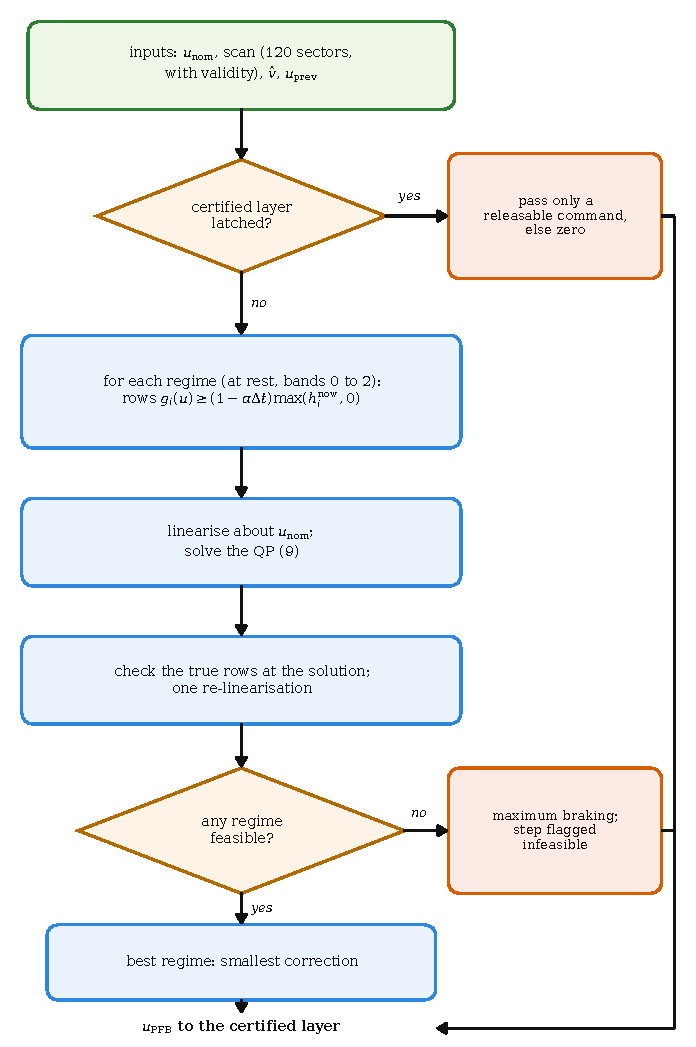
\includegraphics[width=0.62\linewidth]{fig_flowchart.pdf}
\caption{One decision of the PFB filter. While the certified layer is latched, only a command that its restart condition could release passes, and otherwise the output is zero. When it is not latched, the filter builds the barrier rows for each speed regime, linearises them about the nominal command, solves the QP (8), checks the true rows at the solution, and allows one re-linearisation. The regime with the smallest correction is used. If no regime is feasible, the filter commands maximum braking and flags the step. The output goes to the certified layer, which stays active.}
\label{fig:flowchart}
\end{figure}

\begin{figure}[t]
\centering
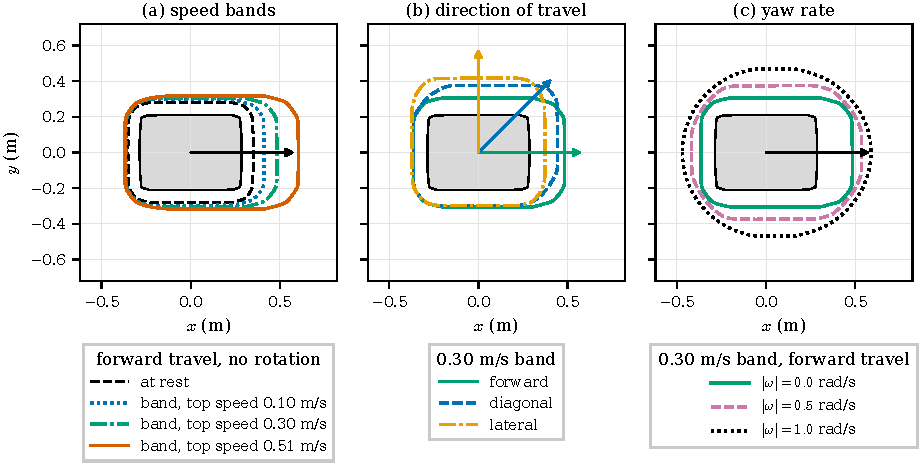
\includegraphics[width=\linewidth]{fig2_field_geometry.pdf}
\caption{Protective fields on the measured footprint (grey). Arrows give the direction of travel. (a) The at-rest field (dashed) and the fields of the three speed bands, with top speeds 0.10, 0.30 and 0.51~m/s, for forward travel without rotation. (b) The field of the 0.30~m/s band for forward, diagonal and lateral travel. (c) The field of the 0.30~m/s band for forward travel at yaw rates of 0, 0.5 and 1.0~rad/s.}
\label{fig:fields}
\end{figure}

\begin{figure}[t]
\centering
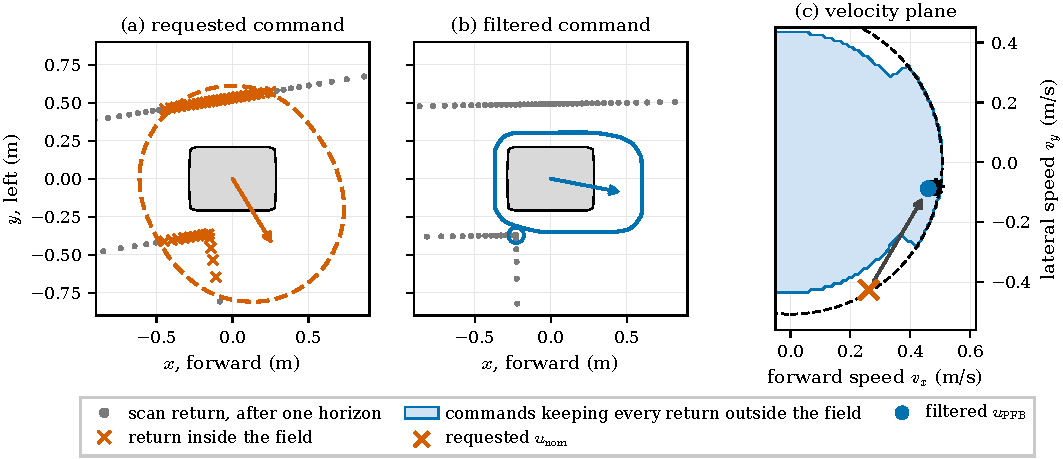
\includegraphics[width=\linewidth]{fig3_pfb_step.pdf}
\caption{One step of the PFB filter, for the step with the largest correction among those in which the requested command violates the field while the robot moves faster than 0.1~m/s. The requested command $u_{\mathrm{nom}}$ is illustrative and comes from a route-following command generator. The scenario is the first narrow-aisle scenario of the tuning set. (a) Robot frame: the protective field (dashed) of the speed regime that the filter selects, drawn for the requested command, and the scan returns as they would lie after one prediction horizon at that command. The crosses are the returns inside the field, each a violated barrier row. (b) The same for the filtered command $u_{\mathrm{PFB}}$: no return is inside its field, and the circle marks the binding return, the one with the least slack. (c) The plane of translational velocity at the filtered yaw rate. The shaded region contains the commands that keep every return outside the field, the dashed arc is the speed limit of the regime, and the dotted circle around the black square, the previously applied command, is the acceleration limiter's one-step envelope. The requested command (cross) lies outside the region, and the filtered command (dot) lies inside it. The requested yaw rate is $-1.45$~rad/s and the filtered yaw rate is approximately 0, so the cross shows the translational part of the requested command.}
\label{fig:step}
\end{figure}

\subsection{Classical controllers}

We evaluate three classical local controllers, each alone and with the PFB beneath. None accounts for the certified fields in its commands, so we call them field-blind. All three receive the same inputs: the route lookahead, the goal and the 120-sector scan stream, and no privileged information. All three run above the same certified layer and actuation limits, and all three use a speed cap derived from the map along the route and the same declared recovery after a latched stop, in which the controller waits a further 1.0 s after the layer's restart delay, then translates at 0.018 m/s for up to 0.30 m in the clearest of 72 body-frame directions, for up to five attempts per episode. Each controller is tuned alone, by the same protocol on the tuning scenarios (Section 5.3), and the filtered version keeps the tuned parameters unchanged.

\emph{B1, holonomic pure pursuit.} The controller steers toward the lookahead point on the route at a cruise speed, with a yaw gain and a slowdown near the goal. It does not use the scan, so it relies on the certified layer to stop it. Its tuned parameters are the cruise speed, yaw gain, goal slowdown and lookahead distance. \cite{coulter1992purepursuit}

\emph{B2, regulated pure pursuit.} The controller follows the route as pure pursuit does and, in the manner of the Nav2 regulated variant, reduces its speed with the curvature of the path and with the proximity of obstacles seen in the live scan. Its tuned parameters are the desired speed, the lookahead time and distance limits, the minimum turning radius, the proximity and approach distances, the minimum speeds and two gains. \cite{macenski2023rpp}

\emph{B3, holonomic dynamic window.} The controller samples commands reachable within one acceleration window and scores the short trajectories they produce for progress, heading and clearance. Its tuned parameters are the maximum speed, the window and simulation times, a safety margin and clearance cap, and three score weights. The first candidate takes the Nav2 DWB defaults. \cite{fox1997dwa}

In the tables, a controller with the filter beneath is written with a suffix, for example B3 + PFB.

\subsection{Planned comparator: a constant-margin beam filter}

To test whether the speed- and direction-dependent field is what removes stops, and not any beam-wise discrete-time barrier, we plan a comparator filter in the manner of the perception-aware filter of~\cite{olayemi2026}. Its field is the footprint's own extent plus one constant margin of 0.10~m, in every speed regime and for every heading and yaw rate of the command. It keeps the same discrete-time row form, the same gain, the same quadratic program and the same actuation limits, and it runs on the same hosts and beneath the same certified layer. The margin was fixed before the comparator was run, and it is not tuned on any set used to evaluate it. In the narrowest aisle it leaves 98.7~mm between the field and the wall for a centred robot. \tbd{the comparator has not been run}


\section{Experimental Design}

This section describes the platform and simulator (5.1), the scenarios (5.2), the tuning of the controllers and the filter gain (5.3), the evaluation protocol (5.4), the metrics (5.5), and the hypotheses and analysis (5.6).

\subsection{Platform and simulation}

The robot is a four-wheel mecanum base derived from the KUKA youBot. It is holonomic: it can translate in any direction and rotate independently. Let $(x, y, \psi)$ be its pose in the world frame, with heading $\psi$, and let $u = (v_x, v_y, \omega)$ be the body twist, with $v_x$ forward, $v_y$ to the left and $\omega$ the yaw rate. The controller issues $u$ at a control period of $\Delta t = 0.05$ s. The pose evolves as

\begin{equation*}
\dot x = v_x \cos\psi - v_y \sin\psi, \qquad
\dot y = v_x \sin\psi + v_y \cos\psi, \qquad
\dot\psi = \omega .
\tag{9}
\end{equation*}

\emph{Wheel kinematics.} Let $r_w = 0.05$ m be the wheel radius, $l = 0.228$ m the half wheelbase and $w = 0.1585$ m the half track, and define the lever arm $L = l + w = 0.3865$ m. With the wheels ordered front-left, front-right, rear-left and rear-right, the wheel angular speeds $\boldsymbol{\varpi} = (\varpi_{\mathrm{fl}}, \varpi_{\mathrm{fr}}, \varpi_{\mathrm{rl}}, \varpi_{\mathrm{rr}})^{\top}$ that realise a twist are given by the mecanum mixing

\begin{equation*}
\boldsymbol{\varpi} = \frac{1}{r_w}\, \mathbf{S}
\begin{pmatrix} v_x \\ v_y \\ L\,\omega \end{pmatrix}, \qquad
\mathbf{S} =
\begin{pmatrix}
1 & -1 & -1 \\
1 & \phantom{-}1 & \phantom{-}1 \\
1 & \phantom{-}1 & -1 \\
1 & -1 & \phantom{-}1
\end{pmatrix}.
\tag{10}
\end{equation*}

A per-wheel sign, fixed by the orientation of the joints in the scene, multiplies each entry and is omitted here. The columns of $\mathbf{S}$ are orthogonal and each has squared norm 4, so $\mathbf{S}^{\top}\mathbf{S} = 4\,\mathbf{I}$, and the twist is recovered from measured wheel speeds by the left inverse

\begin{equation*}
\begin{pmatrix} v_x \\ v_y \\ L\,\omega \end{pmatrix} = \frac{r_w}{4}\, \mathbf{S}^{\top} \boldsymbol{\varpi}.
\tag{11}
\end{equation*}

The rim speed of wheel $i$ is $r_w|\varpi_i|$. Each row of $\mathbf{S}$ combines $v_x$, $v_y$ and $L\omega$ with signs, and the four rows realise every sign pattern of $(v_y, L\omega)$ relative to $v_x$. The fastest wheel therefore has rim speed $\max_i r_w|\varpi_i| = |v_x| + |v_y| + L|\omega|$, and the wheel-speed limit is the polytope

\begin{equation*}
|v_x| + |v_y| + L\,|\omega| \ \le\ f\, v_{\mathrm{rim}},
\tag{12}
\end{equation*}

where $v_{\mathrm{rim}} = 0.617$ m/s is the measured rim-speed ceiling and $f = 0.95$ is the share available to the filter's output. A command that violates (12) is multiplied by a single factor, so that it keeps its direction in all three components and only slows.

\emph{Command limits.} The twist is also confined to an axis box, $|v_x|, |v_y| \le 0.5$ m/s and $|\omega| \le 1.5$ rad/s. The translational pair is scaled along its own direction by the largest factor $s \le 1$ that satisfies $|s v_x| \le 0.5$ and $|s v_y| \le 0.5$, and the yaw rate is clipped separately:

\begin{equation*}
(v_x, v_y) \leftarrow s\,(v_x, v_y), \qquad \omega \leftarrow \mathrm{clip}(\omega, -1.5, 1.5).
\tag{13}
\end{equation*}

An acceleration limiter bounds every change of the applied command with respect to the previously applied one, $u_{k-1}$. The limit on the translational change is isotropic and depends on whether the planar speed decreases:

\begin{equation*}
\big\|(v_x, v_y)_k - (v_x, v_y)_{k-1}\big\| \le
\begin{cases}
a_{\mathrm{dec}}\,\Delta t & \text{if the planar speed decreases},\\
a_{\max}\,\Delta t & \text{otherwise},
\end{cases}
\qquad |\omega_k - \omega_{k-1}| \le \alpha_{\max}\,\Delta t,
\tag{14}
\end{equation*}

with $a_{\max} = 0.5$ m/s$^2$, $a_{\mathrm{dec}} = 1.0$ m/s$^2$ and $\alpha_{\max} = 1.4$ rad/s$^2$. These bounds are not properties of the youBot. They are specified together with the protective fields, so that no speed band can be skipped within one reach time and the robot cannot brake harder than the fields assume. The safety layers use the estimated body velocity $\hat v$, obtained from differenced poses with a low-pass filter of time constant 0.10 s.

\emph{Footprint.} The footprint is a measured table $e(\psi)$, the distance from the body origin to the envelope of every part that can strike an obstacle along each bearing $\psi$, with inscribed and circumscribed radii of 0.209 m and 0.3374 m. Measured quantities are configured at the upper bound of their measurement bracket, because understating a safety footprint is the unsafe direction.

Two scanners of the SICK S300 type sit on diagonally opposite corners and cover 270$^\circ$ each, so that together they see everything outside the outline. The scan plane lies 0.2206 m above the floor. The returns are binned inside the simulator into a policy stream of 36 sectors of 10$^\circ$ and a filter stream of 120 sectors of 3$^\circ$. Each sector carries its minimum range in [0.05, 5.0] m, its bearing and a validity flag. A sector is valid only if its whole extent, from the footprint edge to 1.0 m beyond it, is seen by some sensor. An invalid sector breaches every certified field.

The experiments run in CoppeliaSim 4.10 with the ODE engine at a dynamics step of 0.005 s \cite{rohmer2013vrep}. The engine is a stated condition: in a declared sweep, the same model's heading drift over a 5 m lateral profile was 20.55$^\circ$ under Bullet, 0.47$^\circ$ under ODE and 3.12$^\circ$ under Newton. Scanners are processed inside the simulator and published as one packet per control step. Determinism is claimed within one scene load only. Every run records its commit, host, scene hash and resolved configuration.

\subsection{Scenarios}

\emph{Layouts.} Each scenario is a procedurally generated warehouse hall with perimeter walls and two to four rows of shelving taller than the scan plane. Aisles are stratified by per-side clearance, the gap on each side of a centred robot: narrow [0.1987, 0.2687) m, medium [0.2687, 0.40) m and wide [0.40, 0.80] m. The narrow floor follows a declared rule: it is the smallest clearance at which the at-rest and moving fields of a robot displaced by the committed tracking bound remain clear of the walls, plus a 0.03 m buffer. Start and goal are drawn so that at least 1.5 m of the route lies in an aisle. Every route must be traversable by an oracle tracker that keeps the lowest band's field clear from start to goal. When this check fails, the goal is redrawn, never the layout.

\emph{Obstacles absent from the map.} The central condition of the study is a world that differs from the map. Unmapped obstacles, square boxes of 0.25 to 0.60 m taller than the scan plane, are placed relative to the planned route: the first at an offset uniform on [0, 0.3] m from the route to its nearest surface, any second on [0, 0.6] m. An obstacle is kept only if the robot could pass it within 1.0 m of the route, judged jointly with the obstacles already placed, since the stack does not replan. The planner never sees these obstacles. The scanners and the safety layers do.

\emph{Route and map.} Each layout is rasterised into a 0.05 m grid from which unmapped obstacles are excluded. Cells within the inscribed half-width plus 0.10 m (0.3086 m) of an obstacle are lethal, and a soft cost falls linearly from there to the circumscribed radius plus 0.03 m. An 8-connected A$^{*}$ search finds the cheapest path (Figure~\ref{fig:layouts}). A controller receives a lookahead point 0.8 m ahead on this route and the goal, both in the body frame.

\begin{figure}[t]
\centering
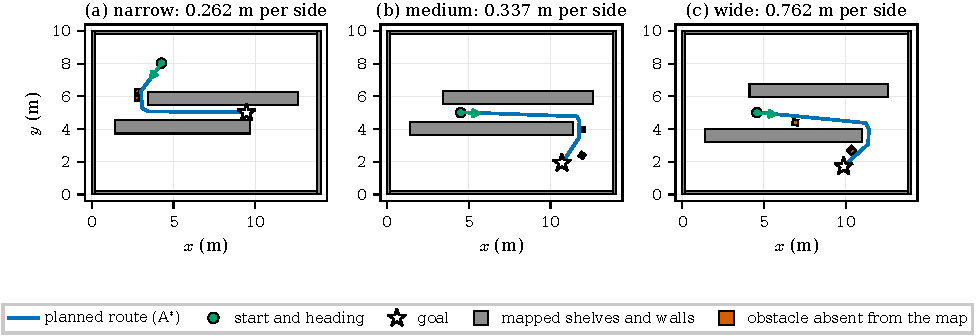
\includegraphics[width=\linewidth]{fig4_layout.pdf}
\caption{Example scenarios, one for each aisle stratum, from the tuning set: (a) narrow, (b) medium and (c) wide, with per-side clearances of 0.262, 0.337 and 0.762~m. Grey rectangles are mapped shelves and walls. Orange squares are obstacles that are absent from the planner's map but present in the world and visible to the scanners. The blue line is the A$^*$ route planned on the map, the green dot with an arrow is the start position and heading, and the star is the goal.}
\label{fig:layouts}
\end{figure}

\emph{Scenario sets.} Layouts are identified by seed, geometry hash and generator hash, regenerated and verified at load, and drawn from disjoint seed ranges (Table~\ref{tab:sets}).

\begin{table}[t]
\caption{Scenario sets. Layouts are drawn from disjoint seed ranges.}
\label{tab:sets}
\centering
\small
\begin{tabular}{lp{5.6cm}p{4.4cm}}
\toprule
Set & Size & Purpose \\
\midrule
Tuning & 60 scenarios (20 per stratum), 633 m planned; 17 contain one or two unmapped obstacles & controller tuning and the gain sensitivity \\
Validation & 180 scenarios, 30 in each of 6 cells (mapped-only and unmapped $\times$ narrow, medium, wide), never trained on & development reporting only; no model or hyperparameter is selected on it \\
Test (sealed) & 300 scenarios: 50 in each of 3 strata $\times$ 2 conditions (mapped-only; one unmapped obstacle on every route); 1,606 m and 1,624 m planned & the confirmatory evaluation, run once \\
\bottomrule
\end{tabular}
\end{table}

The test set was built and locked before any controller was evaluated on it. B1, B2 and B3 alone, and B2 with the filter, were each evaluated once on both of its halves. Test layouts are never used for tuning, debugging, reward design or plots during development.

\subsection{Controller tuning and the filter gain}

Each classical controller is tuned alone, on the tuning scenarios only, by a random search over declared parameter ranges. Every controller receives the same number of candidates. The first candidate of B3 takes the Nav2 DWB defaults. The filtered controller keeps the tuned parameters of its host unchanged, so that a comparison of a controller with and without the filter differs only in the filter.

The filter gain $\alpha$ is frozen at 1.0 s$^{-1}$ for every filtered controller. To show how the stops depend on it, we report a sensitivity analysis on the tuning scenarios for the grid $\alpha \in \{1, 2, 5, 10, 20\}$ s$^{-1}$ with B2 + PFB (Section 6.3). The value 1.0 is the lowest of the grid, and it is not selected as an optimum. The runs use seed 0 on the earlier training host, and are not repeated on the final host.

\subsection{Evaluation protocol}

Each classical controller runs once per scenario, alone and with the filter, within one scene load, so that the two versions see the same layout and the same scan noise. The certified layer is beneath every controller, and the filtered version has the filter above it. A paired comparison uses the same scenarios in the same order, within one scene load. The runs reported here use one run per controller and condition, so they carry no estimate of run-to-run variation beyond the scenario resampling described in Section 5.6, and we state this wherever a result depends on it.

\subsection{Metrics}

Protective stops per 100 m of planned route normalises the number of modeled protective stops by the spatial extent of the task, and it is an operational measure of how often the field intervenes. We use the planned length because it is the same for every controller, so that a controller cannot lower its rate by wandering. The rate is reported beside the success rate, the timeout rate and the mission time, so that a reduction in stops is not read apart from the overall navigation performance. A stop is counted as defined in Section 3.2: a persisting breach and its latch count once, and a breach after a restart counts again. All protective stops are events of the emulated layer. No physical certified scanner is used, and the results make no claim about the behaviour of a certified physical system.

The primary endpoint is protective stops per 100 m of planned route, Eq. (5), pooled over episodes. Stops decided on a corrupted scan packet that the plausibility check replaced by the fail-safe (scan-fault stops) are excluded from the count and reported beside it. The secondary measures are the success rate, the timeout rate and the rate of unrecoverable stops, in which an episode reaches its horizon while a stop is latched and the robot cannot legally move again, so that it is distinguished from a timeout in which the robot was free to move. Contact episodes are decided by the simulator's collision check alone. Stops are also reported per 100 m driven and per 100 m on completed routes only, and the mission time, the share of time latched and the moving speed (the mean speed while not latched) are reported. For the filtered controllers, we report the share of steps on which the filter changed the command and the share on which no regime was feasible. We also report the intervention magnitude, the norm $\|(u_{\mathrm{nom}} - u_{\mathrm{PFB}}) \oslash c\|$ of the correction normalised by the axis ceilings $c$, as its mean and maximum over steps, and the 95th percentile of the filter's computation time per step.

Success and timeouts are reported beside every stop rate, because a controller can lower its stop count by moving little or by stalling.

\subsection{Hypotheses and analysis}

\emph{HF-c} (confirmatory, a family of its own): B2 + PFB triggers fewer protective stops per 100 m of planned route than B2 alone, on the test condition with an unmapped obstacle on every route, strata pooled, each arm run once per scenario. The claim is stop removal only. Success, mission time, latched share and moving speed are reported beside it, descriptively and without inference. All other comparisons are exploratory and are labelled as such: the filter beneath B1 and B3 against each alone, the constant-margin comparator of Section 4.4 \tbd{not yet run}, and the sensitivity to $\alpha$. The classical results in Section 6.1 come from the validation sets and are exploratory. HF-c was evaluated once on the sealed test set, and Section 6.2 reports it.

Table~\ref{tab:comparisons} states what each comparison establishes.

\begin{table}[t]
\caption{What each comparison establishes. HF-c is confirmatory; the others are exploratory.}
\label{tab:comparisons}
\centering
\small
\begin{tabular}{p{4.2cm}p{8.0cm}}
\toprule
Comparison & What it establishes \\
\midrule
B2 vs.\ B2 + PFB & effect of the filter on a classical controller (HF-c) \\
B1, B3 vs.\ each with PFB & whether the effect holds across classical controllers \\
PFB vs.\ constant-margin filter & whether the speed- and direction-dependent field matters \tbd{not yet run} \\
\bottomrule
\end{tabular}
\end{table}

\emph{Estimand and interval.} The estimand is the rate ratio of protective stops, total stops over total planned length per arm, with 0.5 added to each arm's stop count:

\begin{equation*}
\widehat{\mathrm{RR}}_{AB} = \frac{(S_A + 0.5)/\Lambda_A}{(S_B + 0.5)/\Lambda_B},
\tag{15}
\end{equation*}

where $S$ is the pooled stop count and $\Lambda$ the pooled planned length. The interval is a bootstrap of $\log \widehat{\mathrm{RR}}$ in which scenarios are resampled jointly across arms. A classical controller runs once, so its interval has the scenario part alone, with a $t$ quantile on $n - 1$ degrees of freedom. A comparison rejects when the two-sided interval lies wholly below zero on the log scale, and HF-c is tested at the level 0.05. Before the interval was used, its rejection rate at equal true rates was checked on synthetic data, with 150 route pairs, the pilot route lengths and 10,000 replications, over stop rates of 0.5, 1, 2, 5 and 52.8 per 100~m and two levels of difficulty. The gate required the one-sided rejection rate on each side to stay within 0.025 plus three Monte Carlo standard errors, 0.0297. All ten cells passed, the highest rejection rate being 0.0274, and the check was made before the test set was read. The cells at 0.25 stops per 100~m, which lie below the rates of the arms here, were reported and not gated, and a few of them exceeded the bound slightly.

\emph{Power.} At the stop rates seen on the development set, a rate ratio of about 0.009, the power of HF-c at 150 scenarios is close to one, so power did not constrain the test size. We do not weaken the comparison: the rate-ratio interval is reported in any case, and the outcome is labelled inconclusive if the interval includes one. The locked test set will not be enlarged.

\emph{Disclosure.} The test size and HF-c as a confirmatory comparison were fixed before the test set was built or read, but after development-set stop rates had been seen. The comparisons of the filter beneath B1 and B3 were proposed after the test set had been read for other controllers, and nothing about them is confirmatory.

\section{Results}

Subsection 6.1 reports the three field-blind controllers on the validation sets, with one run per controller and condition, and its results are exploratory. Subsection 6.2 reports the confirmatory comparison HF-c on the sealed test set. The remaining subsections are templates, and every result in them is a placeholder until the corresponding run exists. Results carry one of two labels: development set (the tuning scenarios) and held-out (the sealed test set).

\subsection{Field-blind controllers with and without the filter}

\emph{Setting.} Each of B3, B1 and B2 was run alone and with the PFB beneath it on the validation sets: 90 routes without an unmapped obstacle (mapped-only) and 90 routes with an unmapped obstacle on every route, with 30 routes in each of the three aisle strata for each condition. Each cell is a single run with seed 0 on the training host, and the controllers were tuned beforehand on the tuning scenarios. These are exploratory results. They are not the confirmatory comparison HF-c, which uses the sealed test set and is reported in Section 6.2. Contacts and scan-fault stops were zero in every run. The provenance records an unclean working tree, caused by deleted draft files unrelated to the code. Tables~\ref{tab:classical-mapped} and~\ref{tab:classical-unmapped} give the outcomes. Stops are per 100~m of planned route. An episode that ends at an unrecoverable stop has a short driven distance, so the rate per planned length is the comparable quantity. Success and timeouts are reported beside the stops, because a controller can have no stops because it never moves.

\begin{table}[t]
\caption{Field-blind controllers alone and with the PFB on routes without an unmapped obstacle (validation sets, 90 routes, seed 0, one run each; exploratory). Stops are per 100~m of planned route. The columns give the value alone and with the PFB.}
\label{tab:classical-mapped}
\centering
\small
\setlength{\tabcolsep}{4pt}
\begin{tabular}{lcccccccc}
\toprule
 & \multicolumn{2}{c}{Stops per 100~m} & \multicolumn{2}{c}{Success} & \multicolumn{2}{c}{Timeouts} & \multicolumn{2}{c}{Unrecoverable stops} \\
\cmidrule(lr){2-3}\cmidrule(lr){4-5}\cmidrule(lr){6-7}\cmidrule(lr){8-9}
Controller & alone & +PFB & alone & +PFB & alone & +PFB & alone & +PFB \\
\midrule
B3 & 8.35 & 0.0  & 85 & 90 & 0  & 0  & 5  & 0 \\
B1 & 68.3 & 0.0  & 0  & 90 & 0  & 0  & 90 & 0 \\
B2 & 63.3 & 0.43 & 34 & 68 & 10 & 22 & 46 & 0 \\
\bottomrule
\end{tabular}
\end{table}

\begin{table}[t]
\caption{As Table~\ref{tab:classical-mapped}, on routes with an unmapped obstacle on every route (validation sets, 90 routes, seed 0, one run each; exploratory). Stops are per 100~m of planned route.}
\label{tab:classical-unmapped}
\centering
\small
\setlength{\tabcolsep}{4pt}
\begin{tabular}{lcccccccc}
\toprule
 & \multicolumn{2}{c}{Stops per 100~m} & \multicolumn{2}{c}{Success} & \multicolumn{2}{c}{Timeouts} & \multicolumn{2}{c}{Unrecoverable stops} \\
\cmidrule(lr){2-3}\cmidrule(lr){4-5}\cmidrule(lr){6-7}\cmidrule(lr){8-9}
Controller & alone & +PFB & alone & +PFB & alone & +PFB & alone & +PFB \\
\midrule
B3 & 45.7 & 0.0  & 1  & 6  & 75 & 84 & 14 & 0 \\
B1 & 62.5 & 1.2  & 0  & 38 & 0  & 52 & 90 & 0 \\
B2 & 64.0 & 1.6  & 0  & 2  & 4  & 88 & 86 & 0 \\
\bottomrule
\end{tabular}
\end{table}

\emph{Routes without an unmapped obstacle.} B3 is the strongest of the three: alone it completes 85 of 90 routes. Its stops still fall from 8.35 to 0.0 per 100~m with the filter, and its five unrecoverable stops disappear. Its success changes from 85 to 90 of 90, a difference of five routes that one run does not separate from run-to-run variation, so we read it as no loss of success and not as a gain. For B1 and B2 the stops fall from 68.3 and 63.3 to 0.0 and 0.43 per 100~m, and every unrecoverable stop disappears (90 and 46 episodes alone). Success rises from 0 to 90 of 90 for B1 and from 34 to 68 for B2. For B2 the timeouts also rise from 10 to 22.

\emph{Routes with an unmapped obstacle.} The stops fall again: B3, B1 and B2 go from 45.7, 62.5 and 64.0 to 0.0, 1.2 and 1.6 per 100~m, and no unrecoverable stop remains. The routes, however, mostly end in timeouts. With the filter, 84 of 90 routes of B3, 52 of B1 and 88 of B2 time out, against 75, 0 and 4 alone, and the success counts are 6, 38 and 2 of 90 (alone: 1, 0 and 0). The filter removes the stop but does not make a controller route around an obstacle that is missing from its map.

\emph{Time, motion and filter activity.} Table~\ref{tab:classical-time} gives the latched share, the moving speed and the mission time. The latched share falls for the controllers that stop: for B3 from 0.079 to 0.000 of the steps on mapped-only routes and from 0.121 to 0.000 on unmapped routes, for B1 from 0.876 to 0.000 and from 0.865 to 0.002, and for B2 from 0.344 to 0.001 and from 0.596 to 0.002. The moving speed does not rise with it. B3 moves at 0.098 m/s alone and 0.100 m/s with the filter on mapped-only routes, so its stops fall without a loss of speed. B1 moves at 0.180 m/s alone and 0.128 m/s with the filter on mapped-only routes, and at 0.149 and 0.053 m/s on unmapped routes, and B2 at 0.058 and 0.032 m/s on unmapped routes. On the routes that both versions complete, the mission times of B3 and B2 are not longer with the filter (107.2 and 105.1~s for B3 over 85 routes, 158.9 and 147.2~s for B2 over 34 routes). We do not interpret differences of this size from one run. Table~\ref{tab:classical-ratio} gives the share of steps on which the filter changed the command, which ranges from 0.19 to 0.89, the share of steps with no feasible regime, at most 0.004, and the exploratory rate ratio of the stops. For B3 the ratio is 0.0064 [0.0038, 0.0107] on mapped-only routes and 0.0011 [0.0009, 0.0014] on unmapped routes. For B2 it is 0.0076 [0.0032, 0.0181] and 0.0258 [0.0145, 0.0461], and for B1 0.0008 [0.0007, 0.0008] and 0.0200 [0.0110, 0.0366]. These ratios are exploratory, and the intervals for B1 and B3 are narrow because the filtered arm has no or few stops.

\begin{table}[t]
\caption{Latched share, moving speed and mission time beside the stops (validation sets, 90 routes per row, seed 0, one run each; exploratory). The latched share is the share of steps with a latched stop, the moving speed is the distance driven divided by the time not latched, and the mission time is the mean time to the goal over the routes that both versions complete ($n$).}
\label{tab:classical-time}
\centering
\small
\setlength{\tabcolsep}{4pt}
\begin{tabular}{llcccccc}
\toprule
 & & \multicolumn{2}{c}{Latched share} & \multicolumn{2}{c}{Moving speed (m/s)} & \multicolumn{2}{c}{Mission time (s), $n$} \\
\cmidrule(lr){3-4}\cmidrule(lr){5-6}\cmidrule(lr){7-8}
Condition & Controller & alone & +PFB & alone & +PFB & alone & +PFB \\
\midrule
mapped-only & B3 & 0.079 & 0.000 & 0.098 & 0.100 & 107.2 & 105.1, 85 \\
 & B1 & 0.876 & 0.000 & 0.180 & 0.128 & \multicolumn{2}{c}{no common completions} \\
 & B2 & 0.344 & 0.001 & 0.059 & 0.058 & 158.9 & 147.2, 34 \\
\midrule
unmapped & B3 & 0.121 & 0.000 & 0.036 & 0.034 & 156.3 & 144.2, 1 \\
 & B1 & 0.865 & 0.002 & 0.149 & 0.053 & \multicolumn{2}{c}{no common completions} \\
 & B2 & 0.596 & 0.002 & 0.058 & 0.032 & \multicolumn{2}{c}{no common completions} \\
\bottomrule
\end{tabular}
\end{table}

\begin{table}[t]
\caption{Filter activity and the exploratory rate ratio of protective stops (with the PFB over alone) on the same routes (validation sets, 90 routes per row, seed 0, one run each; exploratory). The ratio uses stops per planned length with 0.5 added to each total, and its interval is a bootstrap over routes with a $t$ quantile on 89 degrees of freedom. When one total is zero, the interval reflects the variation of the route lengths and the other arm's stops across routes only.}
\label{tab:classical-ratio}
\centering
\small
\setlength{\tabcolsep}{4pt}
\begin{tabular}{llccc}
\toprule
Condition & Controller & Steps changed by the filter & Steps with no feasible regime & Rate ratio [95\% interval] \\
\midrule
mapped-only & B3 & 0.301 & 0.002 & 0.0064 [0.0038, 0.0107] \\
 & B1 & 0.730 & 0.004 & 0.0008 [0.0007, 0.0008] \\
 & B2 & 0.195 & 0.002 & 0.0076 [0.0032, 0.0181] \\
\midrule
unmapped & B3 & 0.258 & 0.001 & 0.0011 [0.0009, 0.0014] \\
 & B1 & 0.894 & 0.004 & 0.0200 [0.0110, 0.0366] \\
 & B2 & 0.587 & 0.003 & 0.0258 [0.0145, 0.0461] \\
\bottomrule
\end{tabular}
\end{table}

\emph{Interpretation and limits.} B1 alone completes none of its 90 mapped routes, because every route ends in an unrecoverable stop, and B2 alone completes 34. They are weak baselines, and the gain of B1 from 0 to 90 is not evidence about strong planners. B3 is the stronger controller, and its stops fall to zero on both conditions without a loss of success or moving speed on mapped-only routes. The results are exploratory: one run per cell, the validation sets only, seed 0, and controllers tuned on the tuning sets. The mission times are read on routes that both versions complete, so they exclude the routes that only one version completes.

\subsection{Confirmatory comparison HF-c}

HF-c was evaluated once on the sealed test set, on the 150 routes with an unmapped obstacle on every route (1,624~m planned), with B2 and B2 + PFB run on each scenario within one scene load. B2 + PFB triggered 18 protective stops (1.11 per 100~m of planned route) and B2 alone 1,106 (68.1). The rate ratio is 0.0167 with a 95\% interval of [0.0090, 0.0311], which lies wholly below one, so HF-c holds at the declared level of 0.05. No contact and no scan-fault stop occurred in either arm.

Table~\ref{tab:hfc} gives the measures beside the stops. The reduction is not bought by standing still: with the filter B2 drove 880~m against 696~m alone, and its latched share fell from 0.597 to 0.001. It also completes almost none of these routes, with 147 of 150 ending in a timeout, at a moving speed of 0.029 against 0.058~m/s. The claim that HF-c supports is stop removal, and no more.

The other half of the sealed test set, 150 routes without an unmapped obstacle (1,606~m planned), was evaluated the same way and is descriptive, since HF-c does not use it. B2 alone triggered 907 stops (56.5 per 100~m) and B2 + PFB 2 (0.12), a rate ratio of 0.0028 [0.0006, 0.0133], and its success rose from 52 to 110 of 150 routes.

\begin{table}[t]
\caption{HF-c on the sealed test set, B2 alone and with the PFB (150 routes per condition, each arm once per scenario). HF-c is confirmatory on the unmapped condition; the mapped-only rows are descriptive.}
\label{tab:hfc}
\centering
\small
\setlength{\tabcolsep}{4pt}
\begin{tabular}{llcccccc}
\toprule
 & & \multicolumn{2}{c}{Stops per 100~m} & \multicolumn{2}{c}{Success} & \multicolumn{2}{c}{Unrecoverable stops} \\
\cmidrule(lr){3-4}\cmidrule(lr){5-6}\cmidrule(lr){7-8}
Condition & Controller & alone & +PFB & alone & +PFB & alone & +PFB \\
\midrule
unmapped & B2 & 68.1 & 1.11 & 0 & 3 & 146 & 0 \\
mapped-only & B2 & 56.5 & 0.12 & 52 & 110 & 70 & 0 \\
\bottomrule
\end{tabular}
\end{table}

\subsection{Sensitivity to the barrier gain}

The stops of B2 with the filter were measured for $\alpha \in \{1, 2, 5, 10, 20\}$~s$^{-1}$ on the 60 tuning scenarios, each scenario once per grid value, with all values in one scene load, seed 0, on the earlier training host. This is a development-set result from a single run. Table~\ref{tab:alpha} gives it. No contact occurred at any gain.

\begin{table}[t]
\caption{Sensitivity of B2 + PFB to the barrier gain on the tuning scenarios (60 scenarios, seed 0, one run per gain; development set). Fallback steps are the steps on which no regime was feasible.}
\label{tab:alpha}
\centering
\small
\setlength{\tabcolsep}{4pt}
\begin{tabular}{ccccc}
\toprule
Gain $\alpha$ (s$^{-1}$) & Success & Stops per 100~m & Mission time (s) & Fallback steps \\
\midrule
1 & 0.500 & 0.59 & 155.8 & 332 \\
2 & 0.500 & 2.94 & 155.4 & 125 \\
5 & 0.517 & 9.63 & 157.1 & 74 \\
10 & 0.500 & 11.98 & 156.7 & 2,807 \\
20 & 0.517 & 12.93 & 158.1 & 8,142 \\
\bottomrule
\end{tabular}
\end{table}

The stops rise with the gain, from 0.59 per 100~m at 1~s$^{-1}$ to 12.93 at 20~s$^{-1}$, while the success stays between 0.500 and 0.517 and the mission time between 155.4 and 158.1~s. The fallback steps do not follow the gain monotonically, with 332 at 1~s$^{-1}$, 74 at 5 and 8,142 at 20. The declared rule, the fewest stops among the gains within five percentage points of the best success, admits every gain and selects 1.0~s$^{-1}$, which is the lowest of the grid. It is reported as a selection at the edge of the grid, the grid was not extended, and we do not claim that 1.0~s$^{-1}$ is optimal.

\subsection{Constant-margin comparator}

\tbd{not yet run: the comparison of the PFB with a constant-margin beam-wise filter on the same hosts}

\subsection{Remaining stops and timeouts}

The stops and timeouts that remain with the filter are classified from the episode records of the filtered validation runs of Section~6.1, with no further run. A timeout is assigned to a progress class by the share of the planned route that the robot drove by the horizon: under 10\,\%, 10 to 50\,\%, 50 to 90\,\%, or 90\,\% and more. The edges were fixed before any run was read. A stop is attributed to its episode, and the table counts those episodes in which the filter fell back to maximum braking at least once. These are descriptions of the records, exploratory like the runs they come from.

Table~\ref{tab:remaining} gives the classes. The 32 stops that remain are those of B1 (12, all on unmapped routes) and B2 (20, of which 16 are on unmapped routes), and B3 has none. Of these 32, 31 fall in episodes with at least one fallback step. Among the 246 timeouts, none ends below 10\,\% of the route, 86 end between 10 and 50\,\%, 149 between 50 and 90\,\% and 11 beyond 90\,\%. All 84 timeouts of B3 and all 52 of B1 are on unmapped routes, and the 22 timeouts of B2 on mapped-only routes end at 50\,\% of the route or more.

\begin{table}[t]
\caption{Stops and timeouts that remain with the filter, by class (validation sets, 180 routes per row, seed 0, one run each; exploratory). Timeouts are by share of the planned route driven. The braking share is the mean share of steps on which the filter commanded maximum braking, for the timeouts of the class.}
\label{tab:remaining}
\centering
\small
\setlength{\tabcolsep}{4pt}
\begin{tabular}{lcccccc}
\toprule
 & & \multicolumn{3}{c}{Timeouts by share of route driven} & & \\
\cmidrule(lr){3-5}
Controller & Stops (with fallback) & 10--50\,\% & 50--90\,\% & 90\,\% and more & Braking share, 10--50\,\% & Braking share, 50--90\,\% \\
\midrule
B3 + PFB & 0 (0) & 31 & 49 & 4 & 0.255 & 0.086 \\
B1 + PFB & 12 (12) & 22 & 30 & 0 & 0.345 & 0.338 \\
B2 + PFB & 20 (19) & 33 & 70 & 7 & 0.187 & 0.037 \\
\bottomrule
\end{tabular}
\end{table}

The timeouts that end early in the route carry the larger braking share for B3 and B2, 0.255 and 0.187 of the steps against 0.086 and 0.037 for those that end later, while for B1 the two classes are close (0.345 and 0.338).

\subsection{Computational cost}

The decision time per control step was recorded in the filtered and unfiltered validation runs of Section~6.1, with the simulator rendering, on one host (an Intel 24-core CPU, 64~GB of memory and an NVIDIA GeForce RTX 4070). The times are pooled over all steps of a run, and the percentiles are upper bin edges of a histogram of 1~ms bins. Table~\ref{tab:compute} gives them.

\begin{table}[t]
\caption{Decision time per control step in the validation runs (180 routes per run, seed 0; exploratory), in ms. The filtered runs report the filter's own time and the total decision time of controller and filter.}
\label{tab:compute}
\centering
\small
\setlength{\tabcolsep}{4pt}
\begin{tabular}{lccccc}
\toprule
 & \multicolumn{2}{c}{Controller alone} & \multicolumn{3}{c}{Controller with the PFB} \\
\cmidrule(lr){2-3}\cmidrule(lr){4-6}
Controller & median & 95th percentile & filter 95th percentile & decision median & decision 95th percentile \\
\midrule
B1 & 3.2 & 5.3 & 48.2 & 18.6 & 48.4 \\
B2 & 0.4 & 5.1 & 47.1 & 4.0 & 47.4 \\
B3 & 1.4 & 6.4 & 48.4 & 5.2 & 49.8 \\
\bottomrule
\end{tabular}
\end{table}

With the filter, the 95th percentile of the total decision time was 48.4, 47.4 and 49.8~ms for B1, B2 and B3, inside the 50~ms control period, and the filter accounts for nearly all of it. The margin is narrow, and the maximum for a single step reached 80 to 93~ms. In the filtered runs one step, of B3, exceeded the evaluation's own per-step budget of 160~ms. The timings are those of the evaluation runs and not of an isolated measurement of the filter on an otherwise idle host.

\section{Discussion}

Subsections 7.1 to 7.5 are written mainly from the exploratory results of Section~6.1, which come from single runs on the validation sets. The confirmatory comparison HF-c supports the stop removal of B2 on the sealed test set (Section~6.2), and the statements below about B1 and B3 remain exploratory. The limitations are in Subsection 7.6. The section does not repeat the numerical results.

\subsection{Why the filter reduces protective stops}
The certified layer triggers when a valid scan return lies inside the protective field of the speed regime the robot is in. The filter constrains each command so that, over one prediction horizon, no valid return lies inside the field of the regime the robot will be in. A command that would trigger the layer is therefore replaced before the layer sees it, and the layer's own stop is not needed. The results are consistent with this mechanism. With the filter, the protective stops of B1, B2 and B3 fall from 638, 591 and 78 to 0, 4 and 0 on routes without an unmapped obstacle, and from 624, 638 and 456 to 12, 16 and 0 on routes with one (Section~6.1). The share of steps with a latched stop falls to 0.002 or less, and every unrecoverable stop disappears. Across the three controllers the filter changes the command on between 19\,\% and 89\,\% of the steps, but it finds no feasible regime, and so has to brake at the maximum rate, on at most 0.4\,\% of them. Most corrections are therefore ordinary changes of the command and not emergency braking.

These outcomes show that the stops fall, and they do not by themselves show why. The remaining stops, 12 of B1 and 16 of B2 on unmapped routes, are described in Section~6.5. Of the 32 stops that remain across the three controllers, 31 fall in episodes in which the filter fell back to maximum braking at least once. Whether the speed- and direction-dependent geometry of the field is what removes the stops, rather than any barrier margin on the scan, is the question of the constant-margin comparator of Section~4.4 \tbd{constant-margin comparator}.

\subsection{Where it helps most}
The benefit follows the places where a controller stops. Table~\ref{tab:classical-mapped} and the per-stratum counts of the validation sets show two patterns, both from single runs of 30 routes per cell.

First, the condition matters for success but not for stops. The filter removes the stops both on routes without an unmapped obstacle and on routes with one, but success rises substantially only on the first. On mapped-only routes, success rises from 0 to 90 of 90 for B1 and from 34 to 68 for B2, and on unmapped routes it stays at 6, 38 and 2 of 90 for B3, B1 and B2, because most of these routes end in timeouts (Section~7.3).

Second, the aisle stratum matters for the controller whose stops depend on it. The stops of B3 alone on mapped-only routes fall with the aisle width, from 18.98 per 100~m in narrow aisles to 4.42 in medium and 1.26 in wide aisles, and the filter removes them in every stratum. For B3 the success of narrow aisles rises from 25 to 30, and the other strata were already at 30. B1 and B2 stop at 58 to 71 per 100~m in all three strata, and the filter removes them in all three. Success on mapped-only routes rises in every stratum for B2 (from 9 to 21 of 30 in narrow, from 12 to 26 in medium and from 13 to 21 in wide aisles). These patterns are descriptive. With 30 routes per cell and one run, we give no interval by stratum, and we do not claim that the filter helps more in one stratum than in another beyond the places where the controllers stop.

\subsection{Conservatism and excessive braking}
The filter removes the protective stops, but it does not remove the failure to complete the route. On routes with an unmapped obstacle, the share of timeouts rises when the filter is added: from 0 to 52 of 90 for B1, from 4 to 88 for B2 and from 75 to 84 for B3 (Section~6.1). The unrecoverable stops that ended these episodes alone become timeouts with the filter, so a stop is replaced by a robot that is still free to move but does not reach the goal. This is consistent with a controller that does not replan: the stack follows its route, the obstacle is visible in the scan but absent from the map, and the filter keeps the commanded motion out of the field instead of letting it enter. The filter alters the commands, and the controller has no way to use that information to route around the obstacle. The timeouts of the filtered controllers are described in Section~6.5. None of the 246 timeouts ends below 10\,\% of the planned route, and 149 end between 50 and 90\,\%. The analysis of stalls of barrier filters at undesired equilibria~\cite{mestres2026} suggests that such behaviour is a known property of this kind of filter, but it is a continuous-time result and applies to our discrete, latched setting by analogy only.

On routes without an unmapped obstacle, the filter also lengthens the timeouts of one controller: B2 times out on 22 of 90 routes with it against 10 alone, although its success doubles from 34 to 68. The filter is therefore conservative in some situations, and a reduction in stops must be read beside success and timeouts, as the tables do. The moving speed shows the same caution: B1 moves more slowly with the filter, at 0.128 against 0.180~m/s on mapped-only routes and at 0.053 against 0.149~m/s on unmapped routes, and B2 moves more slowly on unmapped routes (0.032 against 0.058~m/s), whereas B3 changes little (Table~\ref{tab:classical-time}). The comparison is confounded, because the alone versions spend most of their time latched and the filtered versions complete more routes. It indicates that part of the gain is bought with a slower approach, which the stop metric does not show.

\subsection{Dependence on the underlying controller}
The effect of the filter is largest for the controllers whose commands take no account of the protective field. B1, B2 and B3 are field-blind, and the filter removes nearly all of their stops, on routes with and without an unmapped obstacle. B3 is the case that carries the evidence: it is the only one of the three that completes most routes alone (85 of 90 mapped-only routes), so its stops are not a symptom of a controller that cannot navigate. Its stops fall from 8.35 to 0.0 per 100~m on mapped-only routes and from 45.7 to 0.0 on unmapped routes, with no loss of success or moving speed on mapped-only routes.

The two cases with the largest gains are weak baselines. B1 alone has an unrecoverable stop on every one of its 90 mapped routes and completes none, and B2 alone completes 34. The rise of B1 from 0 to 90 successes is therefore not evidence about strong planners. For B3 the filter removes the stops on mapped routes with a change in success of the size of run-to-run variation, and on unmapped routes with no improvement in the ability to complete them. These are single exploratory runs on the validation sets with controllers tuned on the tuning sets, so they are exploratory. The confirmatory comparison on the sealed test set confirms the stop removal for B2 only (Section~6.2), and it does not extend to B1 or B3.

\subsection{Fewer stops versus better navigation}
A reduction in protective stops is not an improvement in navigation by itself, and the results show both cases. On routes without an unmapped obstacle, the fall in stops comes with equal or higher success for B1, B2 and B3 (Section~6.1), and the mission times of B2 and B3 on the routes both versions complete are not longer. There the filter improves the stop rate without a cost that the other measures reveal, with the exception of B2, whose timeouts rise from 10 to 22 of 90 routes while its success doubles. On routes with an unmapped obstacle the picture is different. The stops of B3, B1 and B2 fall to 0.0, 1.2 and 1.6 per 100~m, but the timeouts rise to 84, 52 and 88 of 90, and the success counts stay at 6, 38 and 2. B3 shows the point most clearly: with the filter it has no stop at all, and it completes 6 of 90 routes. A stop rate of zero can be reached by a robot that rarely reaches the goal.

Whether replacing an unrecoverable stop by a timeout is an improvement depends on the operational cost of each. An unrecoverable stop is a robot that cannot legally move again, and a timeout is a robot that can still move but has not arrived. The metrics of this paper count both as a failure to complete the route, and we do not claim that the timeout is the cheaper failure. We therefore restrict the claim to stop removal. The filter reduces protective stops on every controller that stops, it does not by itself make a controller complete routes that require avoiding an obstacle missing from its map, and it can lower the moving speed (Section~7.3). The stop rate must be read beside the success rate, the timeouts and the mission time, as the tables do, and a comparison of controllers on the stop rate alone would favour a controller that does not move. The confirmatory comparison reads the same way: in HF-c the stops of B2 fall from 68.1 to 1.11 per 100~m of planned route, while 147 of 150 routes with the filter end in a timeout.

\subsection{Limitations}
Several limitations should be considered when interpreting the results. First, the PFB operates on a modeled representation of the protective-field geometry and switching logic, which may not capture all implementation-specific characteristics of an industrial safety scanner. Second, the filtering condition is evaluated over one prediction horizon and does not establish continuous-time safety or a formal collision-avoidance guarantee, and the barrier is a candidate whose validity is not shown. Third, the effectiveness of the filter depends on the accuracy of the robot motion model and on the validity of the available range measurements. Fourth, the experiments are in simulation, with a static world and a single platform, and reducing modeled protective stops does not imply equivalent behaviour in a physical certified safety system. Fifth, the evidence is exploratory: the results are single runs on the validation sets with controllers tuned on the tuning sets, the confirmatory comparison HF-c covers B2 alone, and the constant-margin comparator has not been run \tbd{update when the comparator exists}. Sixth, B1 and B2 are weak baselines, so the evidence on a strong controller rests on B3. The proposed method is intended as a navigation-level filtering mechanism, not as a replacement for certified safety functions. \tbd{implications of transferring the approach to a physical AMR}

\section{Future Work: Learned Planners}

This paper treats classical local planners only. A learned local planner is the natural next case, and we outline what a study of it would have to test. We report no result for it here.

Filters have been placed in the loop of RL navigation agents, at execution and in training~\cite{wang2022,yang2026cbfrl}, so the setting is not new. The open question for the Protective-Field Barrier is whether training a policy with the filter in the loop gives fewer protective stops than adding the same filter after training, as a separate, labelled post-hoc comparison. The theoretical case for training with a filter~\cite{oh2026} rests on conditions that our filter does not meet: it is conservative, finds no feasible command on a small share of steps and sits above a stateful latch, so we would treat it as motivation and not as a guarantee. Counting and reducing interventions of a safety mechanism has been studied for RL~\cite{thumm2023}, and a stop of a latching layer removes the robot from the learning signal for the length of the latch, so the way a stop enters the reward matters.

A study of this kind would train a Soft Actor-Critic (SAC) local planner \cite{haarnoja2018sac} under one shared learner setup. It would compare a policy trained with the filter in the loop against the same policy class trained without it and filtered afterwards. Proximity shaping would be varied with the filter held fixed, so that the effect of the shaping is not confounded with the effect of the filter. A constraint-based arm that treats stops as a cost \cite{stooke2020pid} would be added, and the constant-margin comparator of Section 4.4 would be run beneath the same policies. The design would declare its seeds and hypotheses before the confirmatory seeds are trained. Every confirmatory seed would train unconditionally. A pilot gate on separate pilot seeds would come first, with a controls check that the zero action fails and a privileged tracker passes. The classical results of this paper, in particular B2 + PFB and B3 + PFB, would serve as the comparators. \tbd{decide the scope and the declared plan of the learned-planner study before it is described further}

\section{Conclusion}

This paper studied a Protective-Field Barrier filter placed between a local controller and an emulated certified safety layer, beneath three field-blind classical planners. The filter turns the controller's command into the closest one that keeps every valid scan return outside the speed-banded protective field the robot will be in, and it leaves the certified layer active and independent.

In exploratory validation runs, the filter removed nearly all protective stops and every unrecoverable stop of pure pursuit, regulated pure pursuit and the holonomic dynamic window planner. For the dynamic window planner, the strongest of the three, the stops per 100 m of planned route fell from 8.35 to 0.0 on routes without an unmapped obstacle and from 45.7 to 0.0 on routes with one. On routes with an unmapped obstacle, most routes ended in timeouts, so the filter removes the stop without making the controller route around an obstacle missing from its map. The confirmatory comparison HF-c on the sealed test set supports the stop removal for regulated pure pursuit, with 18 stops against 1,106 and a rate ratio of 0.0167 [0.0090, 0.0311], although 147 of 150 of its routes still end in a timeout. The constant-margin comparator is pending \tbd{results of the comparator}.

Future work will train a SAC local planner with the filter in the loop and compare it with the same filter added after training (Section 8).


\section*{Acknowledgments}
\tbd{funding and acknowledgements; AI-assistance disclosure as the venue requires}

% Bibliography
\bibliographystyle{unsrt}
\bibliography{references}

\end{document}
